Assemblando insieme le componeneti derivate dalle entità principali, quindi procedendo da un punto di vista dettagliato ad uno generale, otteniamo il modello ER, seguendo l'approccio misto adottato, in questo caso nella fase BOTTOM-UP. 

\noindent\makebox[\textwidth]{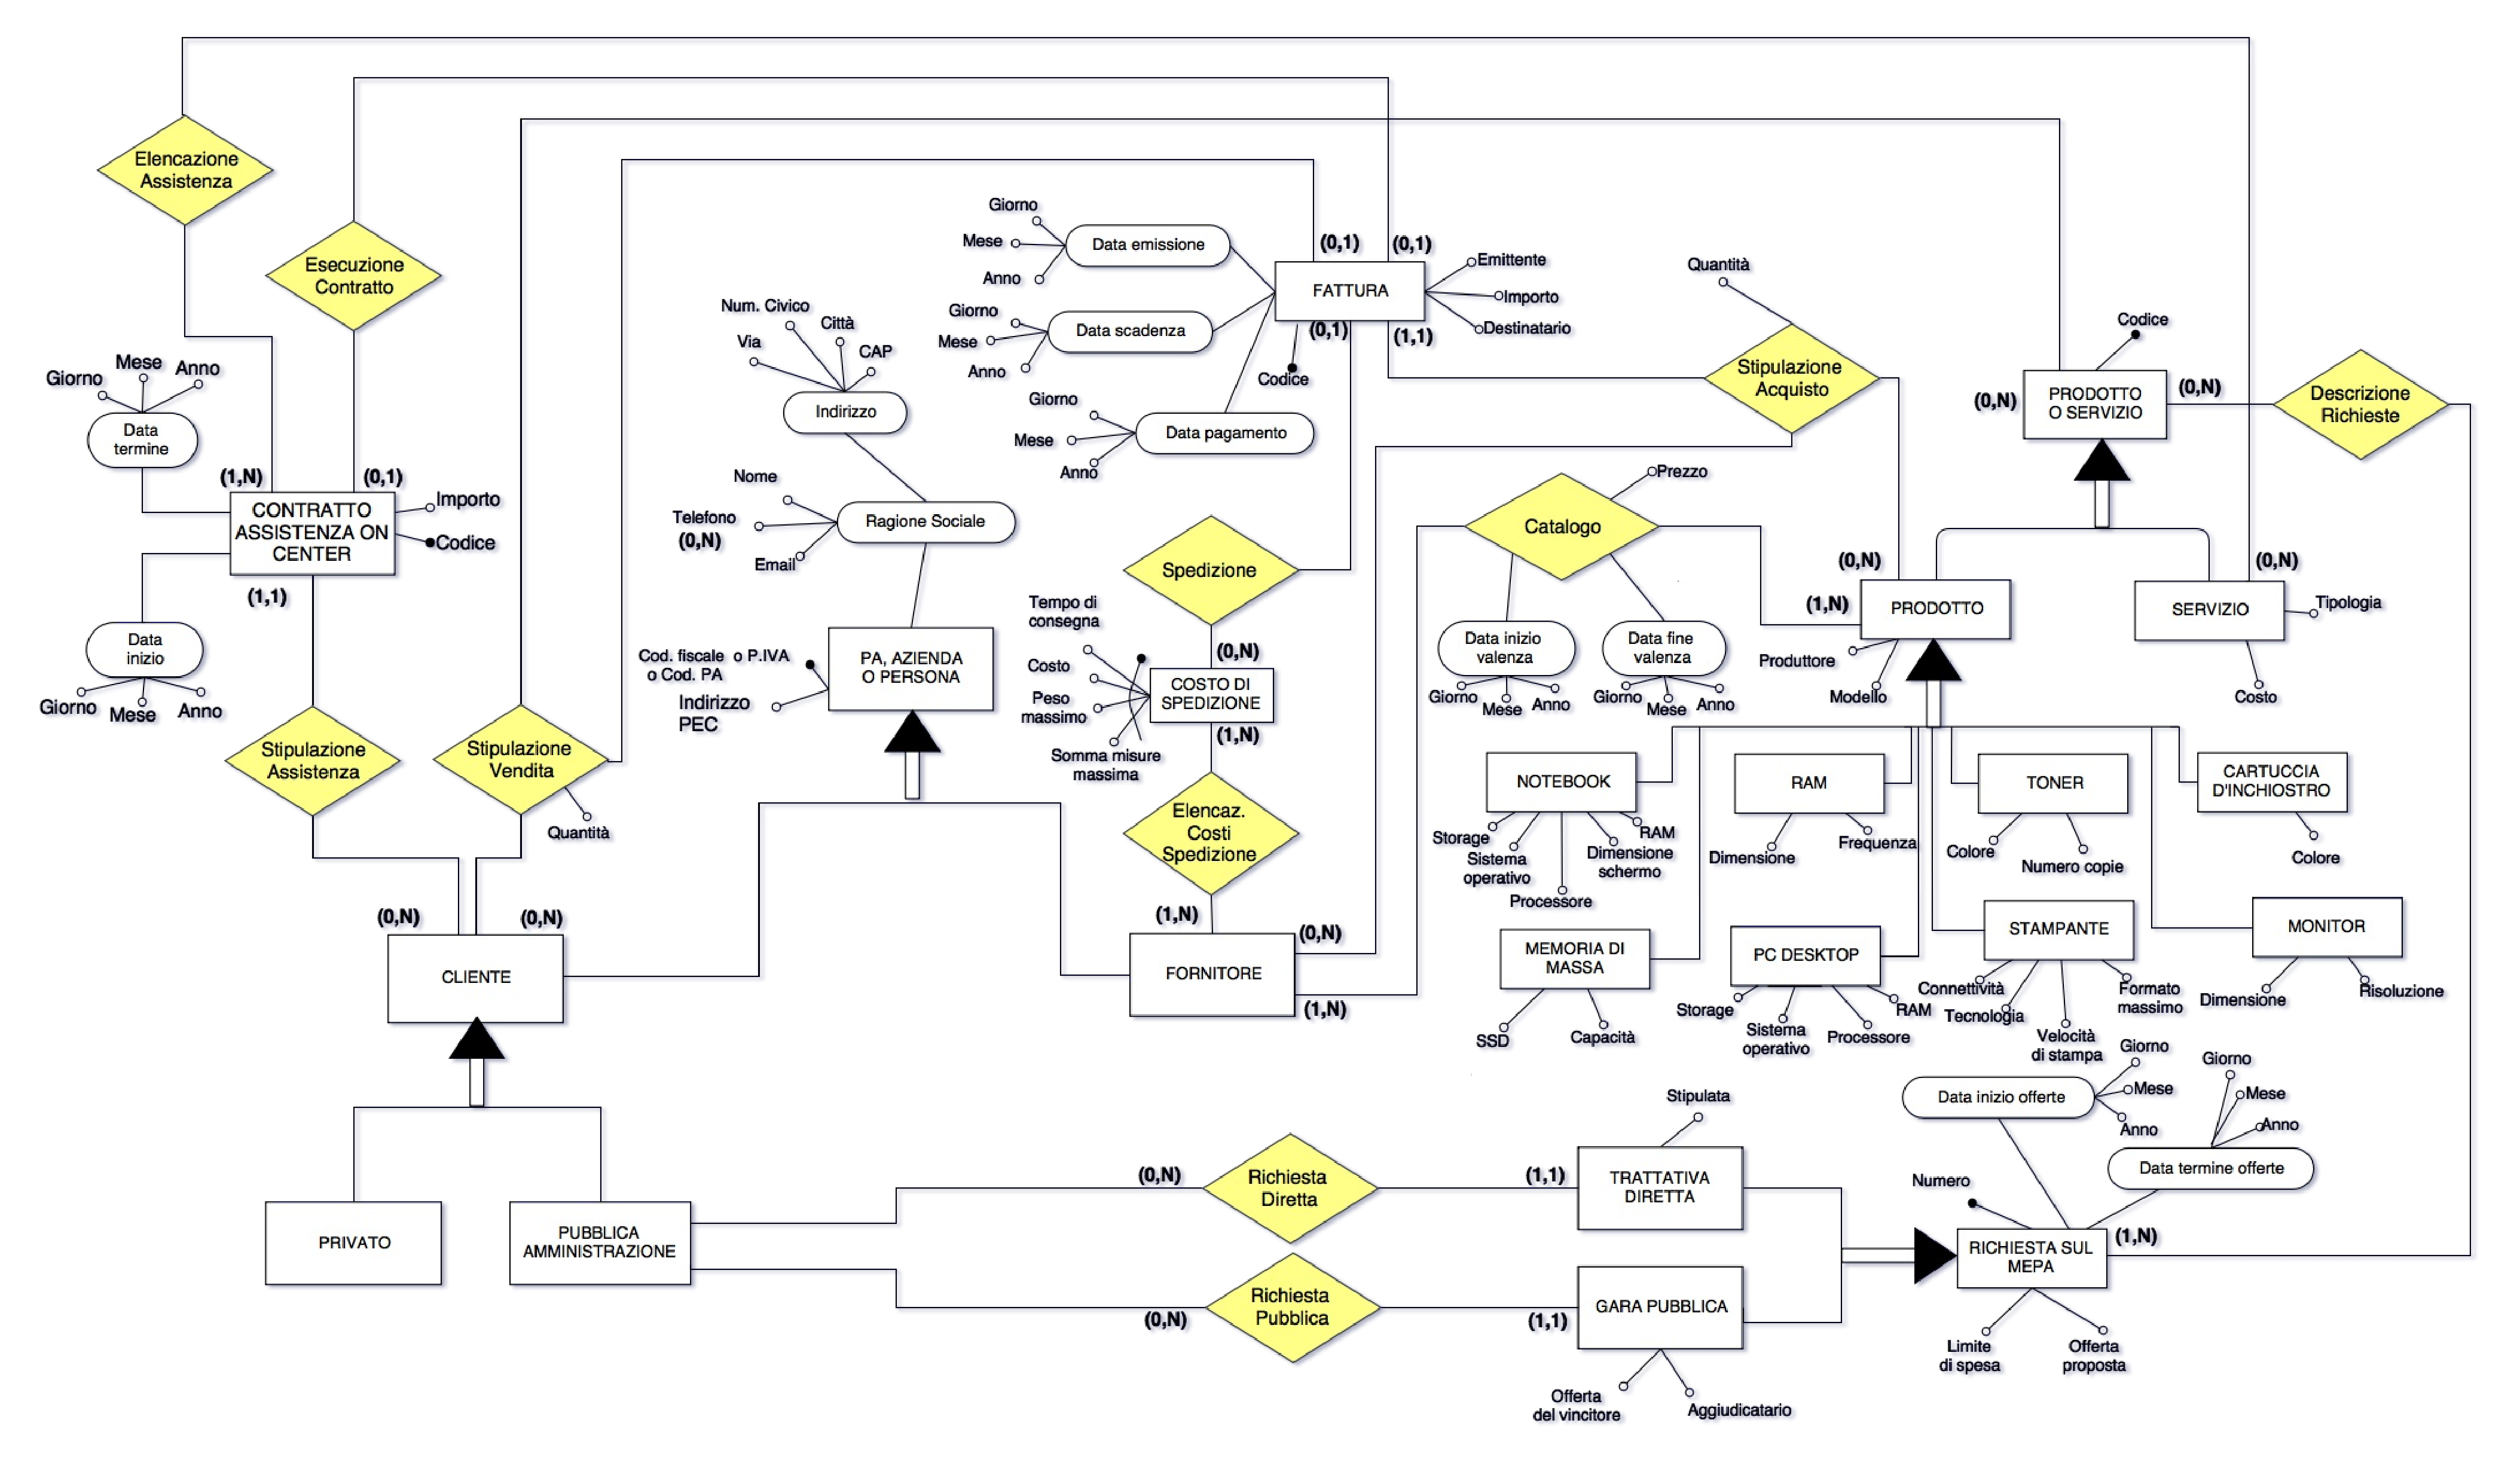
\includegraphics[width=0.9\linewidth]{./immagini/modello_er.pdf}}

